\documentclass[]{article}
\usepackage[spanish.mexico]{babel}
\usepackage[T1]{fontenc}
\usepackage[utf8]{inputenc}
\usepackage{lmodern}
\usepackage[a4paper]{geometry}

%\usepackage{natbib}
\usepackage{cite}





%Plotting

\usepackage{pgfplots}
%(tambien para grafico de barras)

\pgfplotsset{compat=newest}

%###SHARELATEX&&OVERLEAF###
%\pgfplotsset{width=10cm,compat=1.9} 
%\usepgfplotslibrary{external}
%\tikzexternalize 

\usepackage{graphicx}

\usepackage{tikz}
\usepackage[american voltages, american currents,siunitx]{circuitikz}

\title{Proyecto genérico}
\author{Pablo Vivar Colina}
\date{Enero 2019}

\begin{document}

\maketitle

\tableofcontents  % Write out the Table of Contents

\listoffigures  % Write out the List of Figures


\section{Sistemas eléctricos}

\subsection{Leyes de Kirchhoff y circuitos de parámetros concentrados}

Objetivo: enseñar al alumno los modelos matemáticos de los elementos básicos de 2 terminales en el dominio del tiempo $"t"$ y en el dominio de la variable compleja $"s"$.\\

Las leyes de Kirchhoff son las que rigen a los circuitos eléctricos, dichas leyes están basadas en las leyes de la conservación de la carga y de la energía  y se obtienen directamente de las ecuaciones de Maxwell.\\  

\subsubsection{Ecuaciones de Maxwell}

Las ecuaciones de Maxwell como ahora las conocemos son las cuatro citadas anteriormente y a manera de resumen se pueden encontrar en la siguiente tabla:\\


\begin{table}[h!]
	\begin{tabular}{|c|c|c|}
		\hline
		Nombre                               & Forma Diferencial & Forma Integral \\ \hline
		Ley de Gauss                         &     $\vec{\nabla} \cdot \vec{E} = \frac{\rho}{\varepsilon_0}$              &  $\oint_{S} \vec{E} \cdot d\vec{s} = \frac {q}{\varepsilon_0}$              \\ \hline
		Ley de Gauss para el campo magnético &  $\vec{\nabla} \cdot \vec{B} = 0$                 &    $\oint_S \vec{B} \cdot d\vec{s} = 0$            \\ \hline
		Ley de Faraday                       &   $\vec{\nabla} \times \vec{E} = - \frac{\partial \vec{B}}{\partial t}$                &     $\oint_C \vec{E} \cdot d\vec{l} =  - \ { d \over dt } \int_{S} \vec{B} \cdot d\vec{s}$           \\ \hline
		Ley de Ampere Generalizada           &  $\vec{\nabla} \times \vec{B} = \mu_0 \vec{J} + \mu_0 \varepsilon_0  \frac{\partial \vec{E}}{\partial t}$                 &  $\oint_C \vec{B} \cdot d\vec{l} = \mu_0 \int_S \vec{J} \cdot d\vec{s} + \mu_0 \varepsilon_0 \frac{d}{dt} \int_S \vec{E} \cdot d\vec{s}$              \\ \hline
	\end{tabular}
\end{table}

Estas cuatro ecuaciones junto con la fuerza de Lorentz son las que explican cualquier tipo de fenómeno electromagnético. Una fortaleza de las ecuaciones de Maxwell es que permanecen invariantes en cualquier sistema de unidades, salvo de pequeñas excepciones, y que son compatibles con la relatividad especial y relatividad general. Además Maxwell descubrió que la cantidad $c = \frac{1}{\sqrt{\varepsilon_{0} \mu_0}}$ era simplemente la velocidad de la luz en el vacío, por lo que la luz es una forma de radiación electromagnética\cite{EcuacionesMaxwell}.\\

\subsection{Concepto de circuito eléctrico}

Un conjunto de elementos conectados entre si formando trayectorias cerradas por donde puede fluir una corriente eléctrica\\


\begin{figure}[h!]
	\centering
	\begin{circuitikz}
		
		\draw
		    (0,0)to[R,l=$R_1$](3,0)
			(3,0)to[R,l=$R_2$](3,-3)		
			(3,-3)to[R,l=$R_3$](0,-3)
			(0,-3)to[R,l=$R_4$](0,0)
	     ;

	\end{circuitikz}
	\caption{Circuito}
	\label{fig:CircuitoEjemplo}
\end{figure}

\begin{figure}[h!]
	\centering
	\begin{circuitikz}
		
		\draw
		(0,0)to[R,l=$R_1$](3,0)
		(0,-1.5)to[C,l=$C_1$](3,-1.5)		
		(0,-1.5*2)to[L,l=$L_1$](3,-1.5*2)
		(0,-1.5*3)to[V,l=$V_1$](3,-1.5*3)
        (0,-1.5*4)to[vco,l=$G_1$](3,-1.5*4)
        (0,-1.5*5)to[amp,l=$Amp_1$](3,-1.5*5)
        (0,-1.5*6)to[D,l=$D_1$](3,-1.5*6)
        (0,-1.5*7)to[ammeter,l=$A_1$](3,-1.5*7)
  (0,-1.5*8)to[voltmeter,l=$V_1$](3,-1.5*8)
    (0,-1.5*9) to[esource] (3,-1.5*9)
    (1.5,-1.5*9)node {$VM$}
    	[black,fill=black] (3,-1.5*9)circle (.5ex)
		(3,-1.5*9)--(6,-1.5*9)
			(1,-1.5*10) node[op amp] (opamp1) {741}
		%tierra a no invesora
		(1,-15.5)  to  (1,-16) node[ground]{}
		
		;
	     \draw
			[gray,shift={(4,-12)}](0,0)rectangle (2.15,12)
		;
	\end{circuitikz}
	\caption{Muestra de componetes}
	\label{fig:CircuitoSample}
\end{figure}



Podemos apreciar que en el circuito \ref{fig:CircuitoEjemplo} se encuentran 4 resistores en serie, cada uno con una polaridad asociada, con una malla única en la cual circula una corriente $"i"$.\\

Definiciones:\\

\begin{itemize}
	\item Nodo: unión de 2 o mas elementos.
	\item Malla: trayectorias cerradas de los circuitos.
\end{itemize}

\subsection{Leyes de Kirchhoff}

Las leyes de Kirchhoff son dos igualdades que se basan en la conservación de la energía y la carga en los circuitos eléctricos. Fueron descritas por primera vez en 1846 por Gustav Kirchhoff. Son ampliamente usadas en ingeniería eléctrica e ingeniería electrónica.\\

Ambas leyes de circuitos pueden derivarse directamente de las ecuaciones de Maxwell, pero Kirchhoff precedió a Maxwell y gracias a Georg Ohm su trabajo fue generalizado. Estas leyes son utilizadas para hallar corrientes y tensiones en cualquier punto de un circuito eléctrico.\\

\subsubsection{Ley de corrientes de Kirchhoff}

En cualquier nodo, la suma de las corrientes que entran en ese nodo es igual a la suma de las corrientes que salen. De forma equivalente, la suma de todas las corrientes que pasan por el nodo es igual a cero.\\

\begin{equation}
   \sum_{k=1}^n I_k = I_1 + I_2 + I_3+\dots + I_n = 0 
\end{equation}


\subsubsection{Ley de tensiones de Kirchhoff}

En un lazo cerrado, la suma de todas las caídas de tensión es igual a la tensión total suministrada. De forma equivalente, la suma algebraica de las diferencias de potencial eléctrico en un lazo es igual a cero.\cite{LeyesKirchhoff}\\

\begin{equation}
\sum_{k=1}^n V_k = V_1 + V_2 + V_3\dots + V_n = 0
\end{equation}

\subsection{Circuito de parámetros concentrados}

En general, un modelo de parámetros concentrados es un método que simplifica el análisis de un sistema real espacialmente distribuido, mediante la creación de una topología de elementos discretos que aproximan el comportamiento de los componentes distribuidos reales bajo ciertas restricciones.\\

Matemáticamente hablando sirve para reducir las ecuaciones en derivadas parciales espaciales (PDEs) y temporales del continuo (dimensión infinita) de nuestro sistema a un conjunto de ecuaciones diferenciales ordinarias (ODEs) con un número finito de parámetros, del que podemos obtener una solución mucho más fácilmente.\\

\subsubsection{Circuito eléctrico de parámetros concentrados} 

En el caso concreto de sistemas eléctricos este modelo se trata con la teoría de circuitos, en la que se estudian circuitos de parámetros concentrados, asumiendo que los parámetros eléctricos del circuito (resistencia, capacitancia, inductancia) se encuentran confinados a una región pequeña del espacio, en los llamados componentes electrónicos (Resistores, condensadores, inductancias), y que están conectados en un circuito mediante hilos perfectamente conductores.\\

La restricción fundamental al análisis mediante este modelo es que el tamaño del circuito sea mucho menor que la longitud de onda de la señal eléctrica que circule por el propio circuito. En el caso contrario de que el tamaño del circuito sea del mismo orden o mayor que la longitud de onda se deberá tratar el problema de forma más general, con un modelo de parámetros distribuidos (como las líneas de transmisión, cuyo comportamiento dinámico se debe estudiar aplicando directamente las Ecuaciones de Maxwell).\cite{CircuitoParametrosConcentrados}\\ 

\section{Sinusoide}

En matemáticas se denomina sinusoide o senoide a la curva que representa gráficamente la función seno y también a dicha función en sí. Es una curva que describe una oscilación repetitiva y suave.\\

Su forma más básica en función del tiempo (t) es:\cite{Sinusoide}\\

\begin{equation}
y(t) = A\sen(\omega t + \varphi)
\end{equation}

La senoide es importante en física debido al hecho descrito por el teorema de Fourier que dice que toda onda, cualquiera que se sea su forma, puede expresarse de manera única como superposición (suma) de ondas sinosuidales de longitudes de onda y amplitudes definidas. Por este motivo se usa esta función para representar tanto a las ondas sonoras como las de la corriente alterna.\cite{Sinusoide}\\

\subsection{Características}

La sinusoide puede ser descrita por las siguientes expresiones matemáticas:

\begin{equation}
y(x) = A\ {\rm{sen}} (\omega x + \varphi)
\end{equation}

\begin{equation}
y(t) = A\sen(2 \pi f t + \varphi)
\end{equation}

\begin{equation}
y(x) = A\ {\rm{sen}}  (\frac {2\pi }{T}x + \varphi )
\end{equation}

donde:\\

\begin{itemize}
	\item $A$ es la amplitud de oscilación.
	\item $\omega$ es la velocidad angular  \item $\omega = 2\pi f$
	\item $f$ es la frecuencia de oscilación.
	\item $T$ es el período de oscilación  \item  $T = {1}/{f}$
	\item $\omega x$ + $\varphi$ es la fase de oscilación.
	\item $\varphi$ es la fase inicial.
\end{itemize}

\begin{figure}[h!]
	\centering
	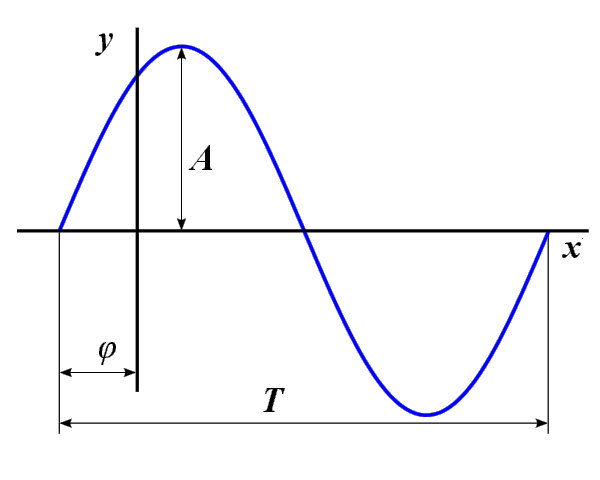
\includegraphics[width=0.6\textwidth]{Imagenes/Alg_sinusoide.png}
	\caption{Parámetros característicos de una forma sinusoidal.}
	\label{fig:parametro_sinusoide}
\end{figure}


%Grafica de 2 parabolas defasadas
\begin{figure}
	\centering
	\begin{tikzpicture}
	\begin{axis}[
	axis lines = left,
	xlabel = $x$,
	ylabel = {$f(x)$},
	]
	%Below the red parabola is defined
	\addplot [
	domain=-10:10, 
	samples=100, 
	color=red,
	]
	{x^2 - 2*x - 1};
	\addlegendentry{$x^2 - 2x - 1$}
	%Here the blue parabloa is defined
	\addplot [
	domain=-10:10, 
	samples=100, 
	color=blue,
	]
	{x^2 + 2*x + 1};
	\addlegendentry{$x^2 + 2x + 1$}
	
	\end{axis}
	\end{tikzpicture}
   \caption{Prueba de pgfplots con etiquetas en ejes y de funciones}
\end{figure}




%GRAFICO DE BARRAS
\begin{figure}[h!]
	\centering
	\begin{tikzpicture}
	\begin{axis}[
	symbolic x coords={A,B,C,D,E,F,G,H,I,J,K},
	xtick=data
	]
	\addplot[ybar,fill=orange] coordinates {
		(A,   291)
		(B,  284)
		(C,   323)
		(D,323)
		(E,339)
		(F,306)
		(G,254)
		(H,282)
		(I,302)
		(J,264)
		(K,272)
	};
	\end{axis}
	\end{tikzpicture}
	\caption{Consumo energía eléctrica [kWh]}
	\label{fig:grafConsumo}
\end{figure}


%Tabla de precios
\begin{figure}[h!]
	\centering
	\begin{tabular}[]{|c|c|c|}
		\hline
		Nombre & Periodo & Energía consumida [kWh]\\
		\hline
		I & 11/8/17-12/10/17 & 323 \\
		
		J & 12/10/17-11/10/17 & 284 \\
		K & 11/12/17-12/2/18 & 291 \\
		
		\hline
	\end{tabular}
	\label{cuadro:ultimosPeriodos}
	\caption{Últimos periodos}
	
\end{figure}


\section{Sinusoide}

En matemáticas se denomina sinusoide o senoide a la curva que representa gráficamente la función seno y también a dicha función en sí. Es una curva que describe una oscilación repetitiva y suave.\\

%Su forma más básica en función del tiempo (t) es:\citep{Sinusoide}\\

\begin{equation}
y(t) = A\sen(\omega t + \varphi)
\end{equation}

%La senoide es importante en física debido al hecho descrito por el teorema de Fourier que dice que toda onda, cualquiera que se sea su forma, puede expresarse de manera única como superposición (suma) de ondas sinosuidales de longitudes de onda y amplitudes definidas. Por este motivo se usa esta función para representar tanto a las ondas sonoras como las de la corriente alterna.\citep{Sinusoide}\\

\subsection{Características}

La sinusoide puede ser descrita por las siguientes expresiones matemáticas:

%\begin{eqnarray}



\begin{equation}
y(x) = A\ {\rm{sen}}\left (\omega x + \varphi \right )
\end{equation}

\begin{equation}
y(t) = A\sen(2 \pi f t + \varphi)
\end{equation}

\begin{equation}
y(x) = A\ {\rm{sen}} \left (\frac {2\pi }{T}x + \varphi \right )
\end{equation}


donde:\\

\begin{itemize}
	\item $A$ es la amplitud de oscilación.
	\item $\omega$ es la velocidad angular  \item $\omega = 2\pi f$
	\item $f$ es la frecuencia de oscilación.
	\item $T$ es el período de oscilación  \item  $T = {1}/{f}$
	\item $\omega x$ + $\varphi$ es la fase de oscilación.
	\item $\varphi$ es la fase inicial.
\end{itemize}

%Cuadrada deterministicas
\begin{figure}[h!]
	\centering
	
	\begin{tikzpicture}
	\begin{axis}[
	axis lines = left,
	xlabel = {t[s]},
	ylabel = {V[V]},
	]
	
	
	\addplot
	[thick=0.1cm,
	domain=0:0.1, 
	samples=100, 
	color=green,
	]
	{(4/3.14159265359)*(sin(2*3.14159265359*1000*x)+(1/3)*sin(3*2*3.14159265359*1000*x)+(1/5)*sin(5*2*3.14159265359*1000*x)};
	%+(1/7)*sin(7*2*3.14159265359*1000*x)+(1/9)*sin(9*2*3.14159265359*1000*x)+(1/11)*sin(11*2*3.14159265359*1000*x)+(1/13)*sin(13*2*3.14159265359*1000*x)+(1/15)*sin(15*2*3.14159265359*1000*x))
	
	%Se añade nota :D
	%\addlegendentry{[1]}
	
	\end{axis}
	\end{tikzpicture}
	\caption{Señal cuadrada unitaria}
	\label{Senalcuadrada20pp}
\end{figure}

%\bibliographystyle{apa}
\bibliography{Referencias.bib}

\end{document}
